\documentclass[tikz,border=7pt]{standalone}
\usepackage{amsmath,pgfplots}
\pgfplotsset{compat=1.18}
\usetikzlibrary{arrows.meta}
\definecolor{ink}{HTML}{21352F}\definecolor{teal}{HTML}{087F7B}
\definecolor{gold}{HTML}{C58B2A}\definecolor{blue}{HTML}{4B77A8}\definecolor{rose}{HTML}{B65A62}
\begin{document}
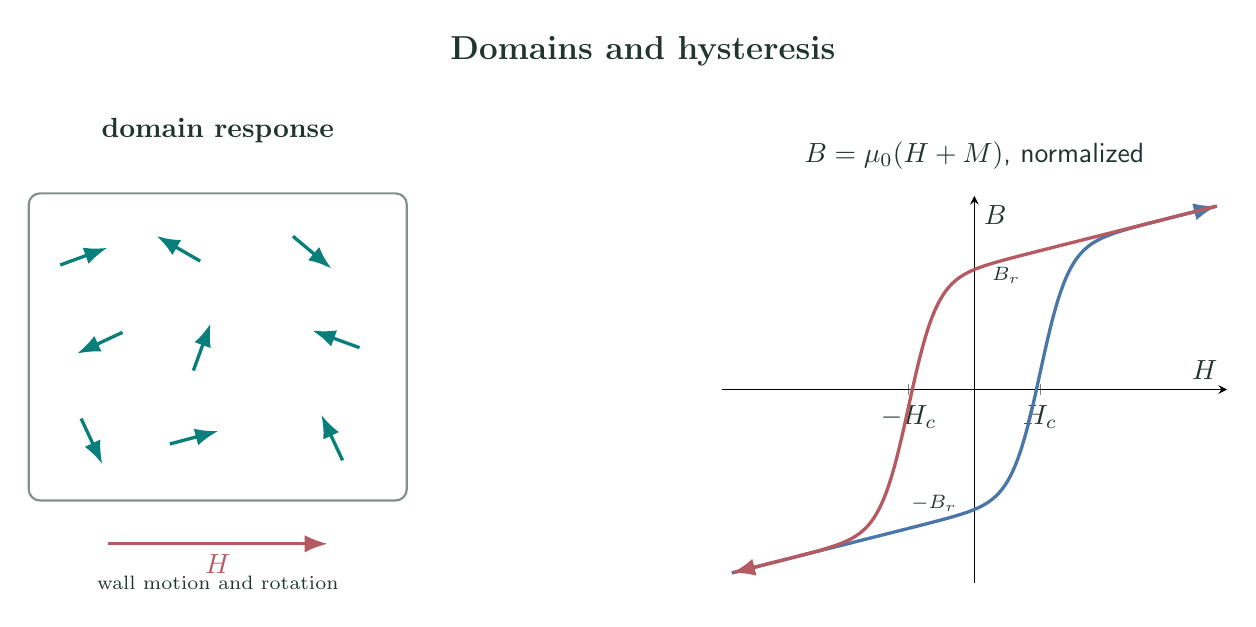
\begin{tikzpicture}[font=\sffamily,text=ink,>=Latex]
\node[font=\bfseries\large] at (0,4.0) {Domains and hysteresis};
\begin{scope}[xshift=-5.4cm,yshift=.1cm]
 \node[font=\bfseries] at (0,2.9) {domain response};
 \draw[rounded corners,ink!55,thick] (-2.4,-1.8) rectangle (2.4,2.1);
 \foreach \x/\y/\a in {-1.7/1.3/20,-.5/1.4/150,1.2/1.35/-40,-1.5/.2/205,-.2/.15/70,1.5/.25/160,-1.6/-1.05/-65,-.3/-1.0/15,1.45/-1.0/115}{
   \draw[->,very thick,teal,rotate around={\a:(\x,\y)}] (\x-.32,\y)--(\x+.32,\y);
 }
 \draw[->,very thick,rose] (-1.4,-2.35)--(1.4,-2.35) node[midway,below] {$H$};
 \node[font=\scriptsize] at (0,-2.85) {wall motion and rotation};
\end{scope}
\begin{axis}[at={(1.0cm,-2.75cm)},anchor=south west,width=8cm,height=6.5cm,xmin=-2.5,xmax=2.5,ymin=-1.9,ymax=1.9,
 axis lines=middle,xlabel={$H$},ylabel={$B$},xtick={-.65,.65},xticklabels={$-H_c$,$H_c$},ytick=\empty,title={$B=\mu_0(H+M)$, normalized}]
 \addplot[blue,very thick,->,domain=-2.4:2.4,samples=260]{.25*x+1.2*tanh((x-.65)/.28)};
 \addplot[rose,very thick,<-,domain=-2.4:2.4,samples=260]{.25*x+1.2*tanh((x+.65)/.28)};
 \node[font=\scriptsize,anchor=west] at (axis cs:.08,1.12) {$B_r$};
 \node[font=\scriptsize,anchor=east] at (axis cs:-.08,-1.12) {$-B_r$};
\end{axis}
\end{tikzpicture}
\end{document}

